\input{../preamble.tex}

\lecturenumber{2}
\title{Kernels}
\version{2.0.0}

\begin{document}

\begin{frame}[plain, noframenumbering]
    \titlepage
\end{frame}

\begin{slide}

    \slidetitle{Aside: Stack In Memory Vs. Stack In Data Structure}

\vspace{-5mm}
\begin{minipage}[t]{0.3\textwidth}
    \vspace{0pt}\par
    \begin{minted}{c}
void functionC(int c) {
    int localC = c + 10;  
    return localC;
}
void functionB(int b) {
    int localB = b + 5;
}
void functionA(int a) {
    int localA = a * 2;  
    functionB(localA);    
}
int main() {
    int x = 5;        
    functionA(x);       
    functionC(x);
    return 0;
}
\end{minted}
\end{minipage}
\hfill
\begin{minipage}[t]{0.5\textwidth}
    \vspace{0pt}\par
        \begin{tabular}{ | p{3cm} | } 
            \hline
            \\ \hline
            \\ \hline
            \\ \hline
            \\ \hline
            \\ \hline
            \\ \hline
            \\ \hline
            \\ \hline
            \\ \hline
            \\ \hline
            \\ \hline
            \\ \hline
            \\ \hline
            \\ \hline
            \\ \hline
        \end{tabular}
\end{minipage}

\end{slide}

\begin{slide}

    \slidetitle{Aside: Java Vs. C}

    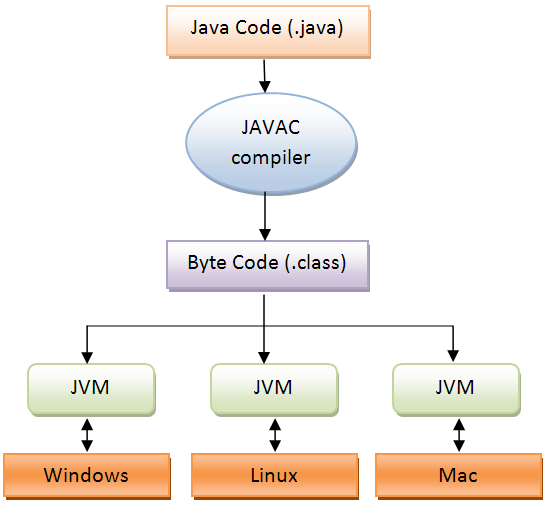
\includegraphics[width=60mm]{java.png}
    
\end{slide}

\begin{slide}

    \slidetitle{Aside: Dynamic (malloc) Vs. Local Variables}

\vspace{-3mm}
\begin{minted}{c}
int* functionA() {
    // stack: Implementation 1
    int num = 42; 
    return &num;  
    
    // heap: Implementation 2
    // int* num = (int*) malloc(sizeof(int));
    // *num = 42;
    // return num;
}

int main() {
    int* ptr = functionA();
    printf("Stack Variable: %d\n", *ptr); 
    // free(ptr);
    return 0;
}
\end{minted}

\end{slide}

\begin{slide}

    \slidetitle{Recap: Physical and Virtual Memory}
    
    \vspace{-5mm}
    (demo: \texttt{local} + \texttt{global} addresses)
    \medskip
    
    (We will talk more on this in greater details later)
    
\end{slide}

\begin{slide}

    \slidetitle{Assignment 1 is Released}

    We will be working with xv6 (A teaching OS developed at MIT).
    \bigskip
    
    The main themes of this assignment are working with processes and becoming comfortable with both kernel and user-level code.
    \bigskip
    
    You will be writing programs at both the user and kernel levels.
    \bigskip
    
    Your TA will be handling all grading for this assignment.
    \bigskip
    
    Please review the assignment, complete at least the setup this week, and visit your TA during tutorial if you encounter any issues.
    \bigskip
    
\end{slide}

\begin{slide}
    
    \slidetitle{Let's Execute This Program and Verify It's ``Hello world''}

    \small \ttfamily
    0x7F 0x45 0x4C 0x46 0x02 0x01 0x01 0x03 0x00 0x00 0x00 0x00 0x00 0x00 0x00
    0x00

    0x02 0x00 0x3E 0x00 0x01 0x00 0x00 0x00 0x78 0x00 0x01 0x00 0x00 0x00 0x00
    0x00

    0x40 0x00 0x00 0x00 0x00 0x00 0x00 0x00 0x00 0x00 0x00 0x00 0x00 0x00 0x00
    0x00

    0x00 0x00 0x00 0x00 0x40 0x00 0x38 0x00 0x01 0x00 0x40 0x00 0x00 0x00 0x00
    0x00

    0x01 0x00 0x00 0x00 0x05 0x00 0x00 0x00 0x00 0x00 0x00 0x00 0x00 0x00 0x00
    0x00

    0x00 0x00 0x01 0x00 0x00 0x00 0x00 0x00 0x00 0x00 0x01 0x00 0x00 0x00 0x00
    0x00

    0xA8 0x00 0x00 0x00 0x00 0x00 0x00 0x00 0xA8 0x00 0x00 0x00 0x00 0x00 0x00
    0x00

    0x00 0x10 0x00 0x00 0x00 0x00 0x00 0x00 0x08 0x08 0x80 0xD2 0x20 0x00 0x80
    0xD2

    0x81 0x13 0x80 0xD2 0x21 0x00 0xA0 0xF2 0x82 0x01 0x80 0xD2 0x01 0x00 0x00
    0xD4

    0xC8 0x0B 0x80 0xD2 0x00 0x00 0x80 0xD2 0x01 0x00 0x00 0xD4 0x48 0x65 0x6C
    0x6C

    0x6F 0x20 0x77 0x6F 0x72 0x6C 0x64 0x0A
    \bigskip

    \normalsize \normalfont Execute using:
    \mintinline{bash}{./hello-world-linux-aarch64}
    
\end{slide}

\begin{slide}

    \slidetitle{Instruction Set Architecture (ISA)}
    
	It's the machine code, or numbers the CPU understands
	\bigskip

    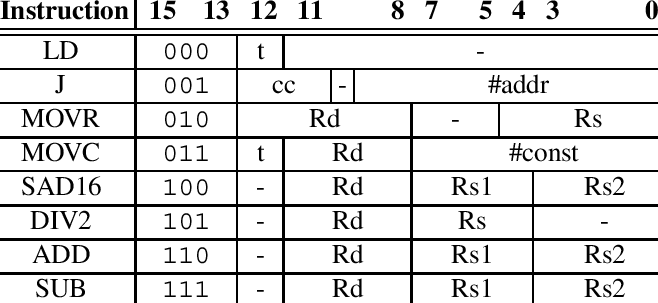
\includegraphics[width=60mm]{instruction-set-architecture.png}
	\medskip
	
	  \texttt{x86-64} (aka \texttt{amd64}): for desktops, non-Apple laptops,
                                          servers
  \medskip

  \texttt{aarch64} (aka \texttt{arm64}): for phones, tablets, Apple laptops
  \medskip

  \texttt{riscv} (aka \texttt{rv64gc}): open-source implementation, similar to
                                        ARM
										
\end{slide}

\begin{slide}
  
  \slidetitle{Our Next Abstraction is a File Descriptor}

  Since our processes are independent, we need an explicit way to transfer data
  \medskip

  \textbf{IPC:} inter-process communication is transferring data between two
  processes
  \bigskip

  \textbf{File descriptor:} a resource that users may either read bytes from
  or write bytes to \newline
  (identified by an index stored in a process)
  \medskip

  A file descriptor could represent a file, or your terminal
\end{slide}

\begin{slide}
  
  \slidetitle{System Calls Make Requests to the Operating System}

    We can represent system calls like regular C functions
    \medskip

    Here are two system calls we need for a basic ``Hello world'' program:
    \bigskip

    \mintinline{c}{ssize_t write(int fd, const void *buf, size_t count);}

    \textbf{Description:} writes bytes from a byte array to a file descriptor

    \leftspace{}\mintinline{c}{fd} - the file descriptor

    \leftspace{}\mintinline{c}{buf} - the address of the start of the byte
    array (called a buffer)

    \leftspace{}\mintinline{c}{count} - how many bytes to write from the
    buffer
    \bigskip

    \mintinline{c}{void exit_group(int status);}

    \textbf{Description:} exits the current process and sets an exit status code

    \leftspace{}\mintinline{c}{status} - the exit status code (0-255)
\end{slide}

\begin{slide}
  
  \slidetitle{A Hypothetical ``Hello world'' Program}

  By convention there's some expected file descriptors:

  \leftspace{}\mintinline{c}{0} - standard input (read)

  \leftspace{}\mintinline{c}{1} - standard output (write)

  \leftspace{}\mintinline{c}{2} - standard error (write)
  \bigskip

  The most basic ``Hello world'' program would start executing the following:

  \begin{minted}{c}
void _start(void) {
  write(1, "Hello world\n", 12);
  exit_group(0);
}
  \end{minted}

\end{slide}

\begin{slide}
  
    \slidetitle{Another Aside: API Tells You What and ABI Tells You How} 

    Application Programming Interface (API) abstracts the details and describes
    the arguments and return value of a function
    \medskip

    \leftspace{}e.g. A function takes 2 integer arguments
    \bigskip

    Application Binary Interface (ABI) specifies the details, specifically how to
    pass arguments and where the return value is
    \medskip

    \leftspace{}e.g. The same function using the C calling convention

    \leftspace{}(arguments on the stack)
  
\end{slide}


\begin{slide}
  
  \slidetitle{Visually How Our ELF File Gets Divided}

  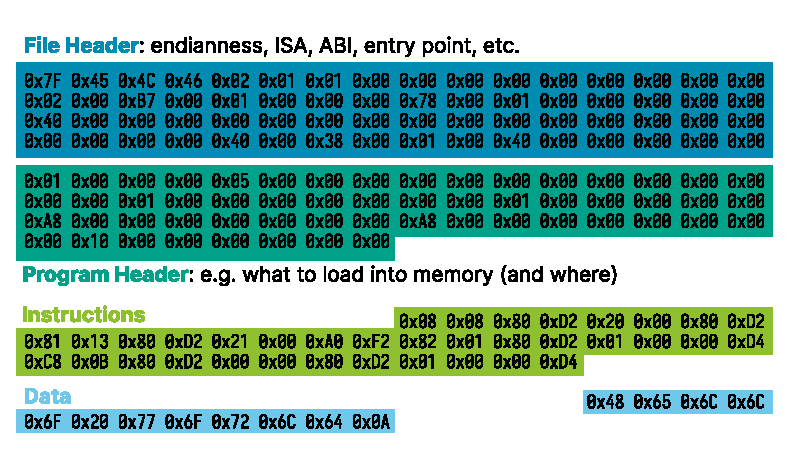
\includegraphics[width=100mm]{hello-world-elf.eps}

\end{slide}

\begin{slide}
  
  \slidetitle{Instructions for ``Hello world'', Using the Linux AArch64 ABI}

  Plug in the 36 bytes for instructions into a disassembler, such as:
  \url{https://onlinedisassembler.com/}
  \bigskip

  Our disassembled instructions:
  \begin{minted}{nasm}
mov  x8, 0x40          #64
mov  x0, 0x01          #1
mov  x1, 0x9C          #156
movk x1, 0x01, lsl 16  #0x10000
mov  x2, 0x0C          #12
svc  0x0
mov  x8, 0x5E          # 94
mov  x0, 0x0           # 0
svc  0x0
  \end{minted}
\end{slide}

\begin{slide}
  
  \slidetitle{The Kernel is a Core Part of Your Operating System}

  \textbf{Kernel mode} is a privilege level on your CPU that gives access
  to more instructions
  \bigskip

  Different architectures have a different name for this mode

  \leftspace{}e.g., this is S-mode on RISC-V

  \bigskip
  \pause

  The kernel is the part of your operating system that runs in kernel mode
  \medskip

  These instructions allow only trusted software to interact with hardware

  \leftspace{}e.g., only the kernel can manage virtual memory for processes
\end{slide}

\begin{slide}
  
  \slidetitle{More Privileged CPU Modes Can Access More Instructions}

  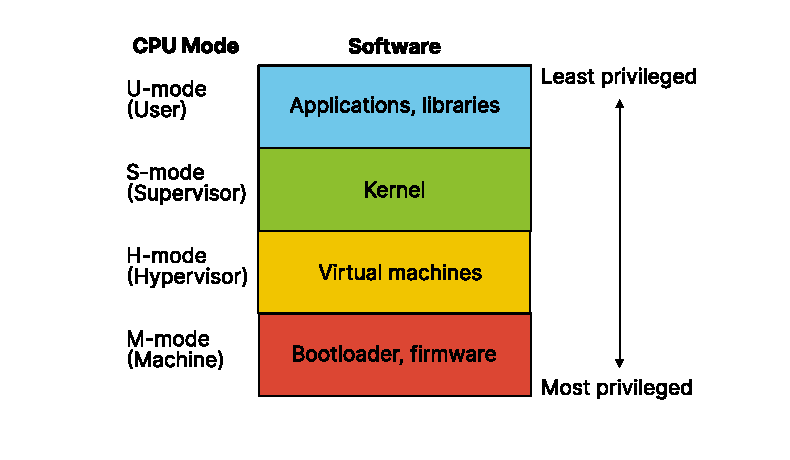
\includegraphics[width=100mm]{cpu-modes.eps}

\end{slide}

\begin{slide}
  
  \slidetitle{System Calls Transition Between User and Kernel Mode}

  \begin{tikzpicture}
    \draw [blue, dashed, thick] (0,0.75)
                                        -- ($(\textwidth - 3pt, 0.75)$);
    \node [blue, anchor=south east] at ($(\textwidth - 3pt, 0.75)$)
          (user) {User space};
    \draw [blue, dashed, thick] (0,-0.75)
                                        -- ($(\textwidth - 3pt, -0.75)$);
    \node [blue, anchor=north east] at ($(\textwidth - 3pt, -0.75)$)
          (kernel) {Kernel space};
    \node [anchor=east] at ($(\textwidth - 3pt, -0)$)
          {\footnotesize (453 total)};
    \node [align=center] at ($(\textwidth/2 - 1.5pt, 0)$)
      {\footnotesize\ttfamily read write open close stat mmap brk pipe clone
                              fork \\
        \footnotesize\ttfamily execve exit wait4 chdir  mkdir rmdir creat mount
                              \\
        \footnotesize\ttfamily init\_module delete\_module clock\_nanosleep
                              exit\_group };
  \end{tikzpicture}
  
  \bigskip
  
  Do you always need root access (sudo) while making a system call?
  
\end{slide}

\begin{slide}
  
  \slidetitle{System Calls Are Traceable}

  We can trace all the system calls a process makes on Linux using the command:

  \leftspace{}\mintinline{bash}{strace <PROGRAM>}
  \medskip

  We can see all the system calls our ``Hello world'' program makes:

  \begin{minted}{console}
execve("./hello_world", ["./hello_world"], 0x7ffd0489de40 /* 46 vars */) = 0
write(1, "Hello world\n", 12)           = 12
exit_group(0)                           = ?
+++ exited with 0 +++
  \end{minted}
  \bigskip

  Now, let's really see what C does...
\end{slide}

\begin{slide}

  \slidetitle{System Calls for ``Hello world'' in C, Finding Standard Library}

  \begin{minted}[fontsize=\scriptsize, escapeinside=]{console}
execve("./hello_world_c", ["./hello_world_c"], 0x7ffcb3444f60 /* 46 vars */) = 0
brk(NULL)                               = 0x5636ab9ea000
openat(AT_FDCWD, "/etc/ld.so.cache", O_RDONLY|O_CLOEXEC) = 3
fstat(3, {st_mode=S_IFREG|0644, st_size=149337, ...}) = 0
mmap(NULL, 149337, PROT_READ, MAP_PRIVATE, 3, 0) = 0x7f4d43846000
close(3)                                = 0
openat(AT_FDCWD, "/usr/lib/libc.so.6", O_RDONLY|O_CLOEXEC) = 3
read(3, "\177ELF\2\1\1\3\0\0\0\0\0\0\0\0\3\0>\0\1\0\0\0000C"..., 832) = 832
lseek(3, 792, SEEK_SET)                 = 792
read(3, "\4\0\0\0\24\0\0\0\3\0\0\0GNU\0\201\336\t\36\251c\324"..., 68) = 68
fstat(3, {st_mode=S_IFREG|0755, st_size=2136840, ...}) = 0
mmap(NULL, 8192, PROT_READ|PROT_WRITE, MAP_PRIVATE|MAP_ANONYMOUS, -1, 0) = 0x7f4d43844000
lseek(3, 792, SEEK_SET)                 = 792
read(3, "\4\0\0\0\24\0\0\0\3\0\0\0GNU\0\201\336\t\36\251c\324"..., 68) = 68
lseek(3, 864, SEEK_SET)                 = 864
read(3, "\4\0\0\0\20\0\0\0\5\0\0\0GNU\0\2\0\0\300\4\0\0\0\3\0\0", 32) = 32
  \end{minted}

\end{slide}

\begin{slide}

  \slidetitle{
    System Calls for ``Hello world'' in C,
  
    Loading Standard Library
  }

  \begin{minted}[fontsize=\scriptsize, escapeinside=]{console}
mmap(NULL, 1848896, PROT_READ, MAP_PRIVATE|MAP_DENYWRITE, 3, 0) = 0x7f4d43680000
mprotect(0x7f4d436a2000, 1671168, PROT_NONE) = 0
mmap(0x7f4d436a2000, 1355776, PROT_READ|PROT_EXEC,
     MAP_PRIVATE|MAP_FIXED|MAP_DENYWRITE, 3, 0x22000) = 0x7f4d436a2000
mmap(0x7f4d437ed000, 311296, PROT_READ,
     MAP_PRIVATE|MAP_FIXED|MAP_DENYWRITE, 3, 0x16d000) = 0x7f4d437ed000
mmap(0x7f4d4383a000, 24576, PROT_READ|PROT_WRITE,
     MAP_PRIVATE|MAP_FIXED|MAP_DENYWRITE, 3, 0x1b9000) = 0x7f4d4383a000
mmap(0x7f4d43840000, 13888, PROT_READ|PROT_WRITE,
     MAP_PRIVATE|MAP_FIXED|MAP_ANONYMOUS, -1, 0) = 0x7f4d43840000
close(3)                                = 0
arch_prctl(ARCH_SET_FS, 0x7f4d43845500) = 0
mprotect(0x7f4d4383a000, 16384, PROT_READ) = 0
mprotect(0x5636a9abd000, 4096, PROT_READ) = 0
mprotect(0x7f4d43894000, 4096, PROT_READ) = 0
munmap(0x7f4d43846000, 149337)          = 0
fstat(1, {st_mode=S_IFCHR|0620, st_rdev=makedev(0x88, 0x1), ...}) = 0
  \end{minted}

\end{slide}

\begin{slide}

  \slidetitle{
    System Calls for ``Hello world'' in C,
  
    Setting Up Heap and Printing
  }

  \begin{minted}{console}
brk(NULL)                               = 0x5636ab9ea000
brk(0x5636aba0b000)                     = 0x5636aba0b000
write(1, "Hello world\n", 12)           = 12
exit_group(0)                           = ?
+++ exited with 0 +++
  \end{minted}
  \bigskip

  The C version of ``Hello world'' ends with the exact same system calls we made
\end{slide}

\begin{slide}
  
  \slidetitle{You Can Think of the Kernel as a Long Running Process}

  Writing kernel code is more like writing library code
  (there's no \texttt{main})
  \bigskip

  The kernel lets you load code (called modules)
  \medskip

  Your code executes on-demand

  \leftspace{}e.g. when it's loaded manually, new hardware, or accessing a
                certain file
  \bigskip

  If you write a kernel module, you can execute privileged instructions

  \leftspace{}and access any kernel data, so you could do anything
\end{slide}

\begin{slide}
  
  \slidetitle{A Monolithic Kernel Runs Operating System Services in Kernel
              Mode}

  \begin{tikzpicture}[box/.style={draw, minimum width=3.5cm,
                                  minimum height=2em,
                                  inner sep=0.5em, node distance=0.5cm}]
    \draw [blue, dashed, thick] (0,0) -- ($(\textwidth - 3pt, 0)$);
    \node [blue, anchor=south east] at ($(\textwidth - 3pt, 0)$)
          (user) {User space};
    \node [blue, anchor=north east] at ($(\textwidth - 3pt, 0)$)
          (kernel) {Kernel space};
    \node [box] (sched) at ($(\textwidth/2 - 1.5pt, -1.25)$)
          {Process Scheduling};
    \node [box, left=of sched] {Virtual Memory};
    \node [box, right=of sched] {IPC};
    \node [box, below=of sched] (dd) {Device Drivers};
    \node [box, left=of dd] {File Systems};
  \end{tikzpicture}
\end{slide}

\begin{slide}
  
  \slidetitle{A Microkernel Runs the Minimum Amount of Services in Kernel
              Mode}

  \begin{tikzpicture}[box/.style={draw, minimum width=3.5cm,
                                  minimum height=2em,
                                  inner sep=0.5em, node distance=0.5cm}]
    \draw [blue, dashed, thick] (0,0) -- ($(\textwidth - 3pt, 0)$);
    \node [blue, anchor=south east] at ($(\textwidth - 3pt, 0)$)
          (user) {User space};
    \node [blue, anchor=north east] at ($(\textwidth - 3pt, 0)$)
          (kernel) {Kernel space};
    \node [box] (sched) at ($(\textwidth/2 - 1.5pt, -1.25)$)
          {Process Scheduling};
    \node [box, left=of sched] {Virtual Memory};
    \node [box, right=of sched] {Basic IPC};
    \node [box] (dd) at ($(\textwidth/2 - 1.5pt, 1.25)$) {Device Drivers};
    \node [box, left=of dd] {File Systems};
    \node [box, right=of dd] {Advanced IPC};
  \end{tikzpicture}
\end{slide}

\begin{slide}
  
  \slidetitle{Other Types of Kernels}

  ``Hybrid'' kernels are between monolithic and microkernels

  \leftspace{}Emulation services to user mode (Windows)

  \leftspace{}Device drivers to user mode (macOS)
  \bigskip

  Nanokernels and picokernels

  \leftspace{}Move even more into user mode than traditional microkernels
  \bigskip

  There's different architectural lines you can draw with different trade-offs
\end{slide}

\begin{slide}

  \slidetitle{Kernel Interfaces Operate Between CPU Mode Boundaries}

  The lessons from the lecture:

  \begin{itemize}
    \item The kernel is the part of the OS that interacts with hardware \newline
          (it runs in kernel mode)
    \item System calls are the interface between user and kernel mode
      \begin{itemize}
        \item Every program must use this interface!
      \end{itemize}
    \item Different kernel architectures shift how much code runs in kernel
          mode
  \end{itemize}

\end{slide}

\begin{slide}

    \slidetitle{Review Qestion: What is the output?}
    
    \inputminted{c}{write_print.c}

\end{slide}

\begin{slide}

    \slidetitle{Review Qestion: True or False}
        
    \bigskip
    
    (1) The write function can be used to print formatted output like printf without additional helper functions.
    
    \bigskip
    
    (2) Calling write(1, "Hello", 5); is functionally equivalent to calling printf("Hello");
    
    \bigskip
    
    (3) printf is a direct system call, whereas write is implemented as a library function.
    
    \bigskip
    
    (4) Calling printf always results in a single system call to write.
    
\end{slide}

\end{document}